\chapter{Экзамен}
\noindent \textit{1. Определение шифра. Шифр простой замены, перестановки, гаммирования. Основные условия криптоанализа.} \\

Отображение $T: X \times K \rightarrow Y$ называется \textbf{шифром}, если $\forall k \in K \\ \exists T^{-1} (y, k) = x$.

Пусть $A = \{ a_1, \ldots , a_m \}$ -- конечный алфавит, $S_m$ -- множество всех подстановок на $A$. Для некоторого натурального $n$ положим $X = A^n$. Если $x = (a_{i_1}, \ldots, a_{i_n})$, $k \in S_m$, то определим \textbf{шифр простой замены} следующим образом:
$$T(x, k) = (k(a_{i_1}), k(a_{i_2}), \ldots, k(a_{i_n})) = y = (b_{i_1}, \ldots, b_{i_n}).$$

Пусть $A = \{ a_1, \ldots , a_m \}$ -- конечный алфавит, $n$ -- натуральное число, $S_n$ -- симметрическая группа подстановок на множестве $\{1, \ldots, n\}$, $X =~A^n$. Если $x = (a_{i_1}, \ldots, a_{i_n})$, $k = \bigl(\begin{smallmatrix}
    1 & \cdots & n \\
    j_1 & \cdots & j_n
  \end{smallmatrix}\bigr) \in S_n$, то \textbf{шифр перестановки} на $X$ определяется следующим образом:
$$T(x, k) = (a_{i_{j_1}}, a_{i_{j_2}}, \ldots, a_{i_n}) = y.$$

Пусть $A = \{ 0, \ldots , m - 1 \}$ -- алфавит, $X =A^n$ -- множество открытых текстов. Рассмотрим кольцо вычетов $\mathbb{Z}_m$. Положим $K = A^n$ и $\forall x \in X, k \in K$, определим \textbf{шифр гаммирования}:
$$y = T(x, k) = (x + k) \pmod m,$$

\noindent где сложение происходит в кольце $\mathbb{Z}_m$.

\newpage
\textbf{Основные условия криптоанализа}:

\noindent 1. Известен шифртекст $y$, один или несколько. Задачи:

а) Нахождение $T$ -- преобразования зашифрования;

б) Нахождение $T, T^{-1}, x$ -- дешифрование по шифртексту.

\noindent 2. Известны одна или несколько пар $(x, y)$. Определить $T(T^{-1})$ и найти $k$ -- ключ шифрования.

\noindent 3. Известны $T(T^{-1})$, один или несколько шифртекстов y. Найти:

а) x -- бесключевое чтение;

б) k, x -- дешифрование по шифртексту при известной шифрсистеме.

\noindent 4. Известны $T, T^{-1}, (x, y)$. Найти $k$.

а) Известны особые x -- атака выбранного открытого текста;

а) Известны особые y -- атака с использованием шифртекста.

\noindent 5. Известны $T, T^{-1}$, шифртекст $y$ или пары $(x, y)$, некоторая форма преобразования $T(.,k)$, но неизвестны $k$ и $T^{-1}(., k)$ -- системы с открытым ключом (Диффи и Хеллман, 1976 г.) \\

\noindent \textit{2. Теоретическая стойкость по Шеннону. Практическая стойкость. Пример совершенного шифра.} \\

\textbf{Теоретическая стойкость} (совершенная секретность) -- Система является безопасной против атак противника с неограниченным временем и ресурсами.

\textbf{Практическая стойкость} (вычислительная) -- Система является безопасной против атак противника в ограниченный период времени с ограниченными ресурсами.

Шеннон определил совершенную секретность условием:
$$P(x | y) = P(x)\ \ \forall x \in X, y \in Y,$$
\noindent где $X, Y$ -- множества открытых сообщений и возможных шифртекстов.

\textbf{Пример совершенного шифра} -- шифр гаммирования, в котором равновероятный ключ имеет ту же длину, что и открытый текст. Пусть $X = \{0, 1\},\ Y = \{0, 1\}, K = \{0, 1\}$, $T(x, k) = (x \oplus k) \pmod 2$, \\ $T^{-1}(y, k) = (y \oplus k) \pmod 2$, $X \sim \begin{pmatrix}
    0 & 1 \\
    p & q
  \end{pmatrix}$, $q = 1 - p$, $Y \sim \begin{pmatrix}
    0 & 1 \\
    0.5 & 0.5
  \end{pmatrix}$, $K \sim \begin{pmatrix}
    0 & 1 \\
    0.5 & 0.5
  \end{pmatrix}$, $P(Y|X) = \frac{P(X, Y)}{P_X (X)} = \begin{pmatrix}
    y/x & 0 & 1 \\
    0 & 0.5 & 0.5 \\
    1 & 0.5 & 0.5 
  \end{pmatrix}$.

По формуле Байеса:
$$P(X = x | Y = y) = \frac{P_X(x) P(y | x)}{P(y)} = \frac{P_X(x)}{\frac{1}{2} 2} = P_X(x).$$

\noindent \textit{3. Метод полного перебора, его средняя трудоемкость. Параллельное опробование с помощью случайно выбираемого на каждом шагу ключа.} \\

Пусть известны $T, T^{-1}, (x, y)$, а ключ неизвестен. \textbf{Методом полного перебора} называется поиск решения уравнения $T(x, k) = y$ перебором по всем $k \in K,\ \ |K| < \infty$.

Определим случайные величины: $\tau$ -- количество опробований ключа включительно до момента обнаружения, $\xi_i = [$ключ на $i$-м месте$]$. Ключ равновероятен, тогда $P(\xi_i = 1) = \frac{1}{|K|}$ для всех $i = \overline{1, |K|}$. \textbf{Средняя трудоёмкость МПП}:
$$\mathbb{E} \tau = \sum_{i = 1}^{|K|} i P (\xi_i = 1)= \frac{1}{|K|} \sum_{i = 1}^{|K|} i = \frac{|K|(|K| + 1)}{|K| \cdot 2} = \frac{|K| + 1}{2}.$$

Пусть параллельно работают $N$ машин. Если $t$ -- число шагов работы машин, то $Nt$ -- число опробований. Число тактов опробования -- случайная величина $\eta$. Аналогом является задача о размещениях: в каждую из $|K|$ ячеек может попасть от $0$ до $N$ частиц. Вероятность того, что из комплекта $i$ ни одна частица не попадёт в данную ячейку, равна $q = (1 - \frac{1}{|K|})^N$. Первое попадание в данную ячейку на комплекте с номером $t$, означающее, что ключ получен, имеет вероятность $P(\eta = t) = q^{t-1}(1-q)$ -- с.в. $\eta$ имеет геометрическое распределение. Тогда \textbf{средняя трудоёмкость МПП при параллельном опробовании} равна: 
$$\mathbb{E}\eta = \frac{1}{1 - q} = \frac{1}{1 - (1 - \frac{1}{|K|})^N} \approx \big \{ N << |K| \big \} \approx \frac{1}{1 - 1 + \frac{N}{|K|}} = \frac{|K|}{N}.$$

\noindent \textit{4. Аналитический метод криптоанализа. Треугольные системы и их решение. Линейные системы. Сложность решения методом Гаусса.} \\

Пусть $K = K_1 \times K_2 \times \ldots \times K_r$, $x = (x_1 x_2 \ldots x_s)$, $y = (y_1 y_2 \ldots y_s)$, $x_i, y_i \in A$. \textbf{Идея аналитического метода} заключается в том, чтобы записать систему уравнений и решить её относительно ключа:

\begin{equation*}
    \begin{cases}
    y_1 = f_1 (x_1, \ldots, x_s, k_1, \ldots, k_r) \\
    \cdots \\
    y_s = f_s (x_1, \ldots, x_s, k_1, \ldots, k_r) 
    \end{cases}
\end{equation*}

\noindent Известны $f_i$ и $(x, y)$.

Пусть эту систему можно преобразовать к \textbf{треугольной системе}:

\begin{equation*}
    \begin{cases}
    g_1 (x, y) = h_1 (x, y, k_1) \\
    g_2 (x, y) = h_2 (x, y, k_1, k_2) \\
    \cdots \\
    g_r (x, y) = h_r (x, y, k_1, \ldots, k_r) 
    \end{cases}
\end{equation*}

\noindent 1. Опробуем $k_1 \in K_1$, число опробований $\le |K_1| \Rightarrow$ восстанавливаем $k_1$.

\noindent 2. Опробуем $k_2 \in K_2$, число опробований $\le |K_2| \Rightarrow$ восстанавливаем $k_2$.

\noindent \ldots

\noindent r. Опробуем $k_r \in K_r$, число опробований $\le |K_r| \Rightarrow$ восстанавливаем $k_r$. \\

\noindent Таким образом, сложность $\le |K_1| + |K_2| + \ldots + |K_r|$. \\

Пусть имеется \textbf{линейная система}:

\begin{equation*}
    \begin{cases}
    b_{11} k_1 + b_{12} k_2 + \ldots + b_{1r} k_r = g_1 (x, y)  \\
    b_{21} k_1 + b_{22} k_2 + \ldots + b_{2r} k_r = g_2 (x, y)  \\
    \cdots \\
    b_{r1} k_1 + b_{r2} k_2 + \ldots + b_{rr} k_r = g_r (x, y)  \\
    \end{cases}
\end{equation*}

\noindent Методом Гаусса решается за $\sum_{k=1}^r k^2 = \frac{r(r + 1)(2 r + 1)}{6} \approx \frac{r^3}{3}$ операций. \\

\noindent \textit{5. Регистр сдвига с нелинейной обратной связью. Линейная сложность. Условия регулярности (теорема с доказательством).} \\

Последовательность $\gamma$ называется \textbf{линейной рекуррентной последовательностью} (ЛРП) порядка $r > 0$ над $GF(2)$, если она описывается \textbf{законом рекурсии}:
$$\gamma_{n+r} = \sum_{i=0}^{r-1} \alpha_i \gamma_{r+n-i},\ \ n = 0,1,\ldots$$
\noindent $\alpha_i \in GF(2),\ i=1,\ldots,r-1,\ \alpha_0 = 1$ и все операции выполняются в поле $GF(2)$.

\textbf{Нелинейная рекуррентная последовательность} (НЛРП) определяется выражением:
$$\gamma_{n+r} = f (\gamma_n, \gamma_{n+1}, \ldots, \gamma_{n+r-1}),\ \ n = 0,1,\ldots$$

\textbf{Регистр сдвига с нелинейной обратной связью} (НЛРС) выглядит следующим образом:

\medskip

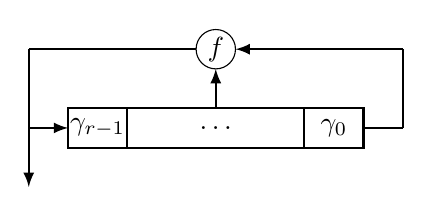
\begin{tikzpicture}[>=latex]
    {\centering
    
    \draw[thick] (0, 0) rectangle node[midway] {$\gamma_{r-1}$} (0.75, 0.5);

    \draw[thick] ( 0.75, 0) rectangle node[midway] {$\ldots$} (3 * 0.75 + 0.75, 0.5);
    \draw[thick, ->] (0.375 + 2 * 0.75, 0.5) -- (0.375 + 2 * 0.75, 1);

    \draw[thick] (4 * 0.75, 0) rectangle node[midway] {$\gamma_0$} (4 * 0.75 + 0.75, 0.5);

    \draw[thick, <-] (0,0.25) -- (-0.5,0.25);
    \draw[thick, <-] (-0.5, -0.5) -- (-0.5,1.25);
    \draw[thick, -] (-0.5,1.25) -- (1.875 - 0.25,1.25);
    
    \draw (1.875, 1.25) circle (0.25) node {$f$};
    
    \draw[thick, -] (3.75, 0.25) -- (4.25,0.25);
    \draw[thick, -] (4.25, 0.25) -- (4.25,1.25);
    \draw[thick, <-] (1.875 + 0.25,1.25) -- (4.25,1.25);

    }
\end{tikzpicture}

\medskip

Нелинейный регистр сдвига называется \textbf{регулярным}, если порождаемая им выходная последовательность $\gamma$ периодична при любом начальном заполнении регистра.

\textbf{Условие регулярности}: если НЛРС регулярен, то для любого начального заполнения существует ЛРС (вида) размера $v$ ($v \ge r$) такой, что порождаемая им последовательность совпадает с последовательностью, порождаемой при этом начальном заполнении НЛРС.

\textbf{Доказательство}: НЛРС регулярен $\Rightarrow$ при любом начальном заполнении последовательность $\gamma$ периодична $\Rightarrow$ ЛРС вида $\gamma_{n+T} = \gamma_n,\\ n = 0, 1, \ldots$ порождает ту же последовательность. \\

\noindent \textit{6. Метод “встреча посередине”. Трудоемкость метода. Пример реализации метода “встреча посередине”.} \\

Пусть даны два шифра: $T_1 (x, k_1)$ и $T_2 (z, k_2)$. Положим
$$y = T_2 (T_1 (x, k_1), k_2)$$

\noindent \textit{9. Первая теорема Шеннона (теорема с доказательством).} \\



\noindent \textit{10. Вторая теорема Шеннона (теорема с доказательством).} \\


